\documentclass[12pt]{article}

\usepackage{fullpage}
\usepackage{multicol,multirow}
\usepackage{tabularx}
\usepackage{ulem}
\usepackage[utf8]{inputenc}
\usepackage[russian]{babel}
\usepackage{graphicx}
\DeclareGraphicsExtensions{.pdf,.png,.jpg,.svg}
\begin{document}
	
	\section*{Лабораторная работа №\,3 по курсу дискртного анализа: Исследование качества программ}
	
	Выполнил студент группы М8О-208Б-20 \textit{Ядров Артем}.
	
	\subsection*{Условие}
	
	Кратко описывается задача: 
	\begin{enumerate}
		\item Для реализации словаря из предыдущей лабораторной работы необходимо провести исследование скорости выполнения и потребления оперативной памяти.
	\end{enumerate}
	
	\subsection*{Метод решения}
	
	зучение утилит для исследования качества программ таких как gcov, gprof, valgrind, и их использование для оптимизации программы.
	
	\subsection*{Valgrind}
	
	Valgrind — инструментальное программное обеспечение, предназначенное для отладки использования памяти, обнаружения утечек памяти, а также профилирования.
	
	В ходе выполнения лабораторной работы утилита будет использована исключительно для отладки использования памяти.
	
	\begin{small}
		\begin{verbatim}
			==10756== 
			==10756== HEAP SUMMARY:
			==10756==     in use at exit: 125,255 bytes in 56 blocks
			==10756==   total heap usage: 145 allocs, 89 frees, 278,123 bytes allocated
			==10756== 
			==10756== LEAK SUMMARY:
			==10756==    definitely lost: 320 bytes in 5 blocks
			==10756==    indirectly lost: 2,055 bytes in 45 blocks
			==10756==      possibly lost: 0 bytes in 0 blocks
			==10756==    still reachable: 122,880 bytes in 6 blocks
			==10756==         suppressed: 0 bytes in 0 blocks
			==10756== Rerun with --leak-check=full to see details of leaked memory
			==10756== 
			==10756== For lists of detected and suppressed errors, rerun with: -s
			==10756== ERROR SUMMARY: 0 errors from 0 contexts (suppressed: 0 from 0)
		\end{verbatim}
	\end{small}

	Как видим, Valgrind не обнаружил утечек памяти. Можно спать спокойно. Однако, существует существенный недостаток утилиты: она не отслеживает выход за границы выделенной памяти. Поэтому я стараюсь использовать средство fsanitize.
	
	\subsection*{gprof}
	
	Gprof - это инструмент для профилирования программы. Мы можем отследить, где и сколько времени проводила программа, тем самым выявляя слабые участки.
	
	Возьмем достаточно большой тест и применим утилиту gprof.
	
	\begin{small}
		\begin{verbatim}
			Flat profile:
			
			Each sample counts as 0.01 seconds.
			%   cumulative   self              self     total           
			time   seconds   seconds    calls  ms/call  ms/call  name    
			75.00      0.24     0.24     3044     0.08     0.09  DeserializeRecursive(std::basic_ifstream<char, std::char_traits<char> >&)
			12.50      0.28     0.04     3124     0.01     0.01  SerializeRecursive(TAVL<std::__cxx11::basic_string<char, std::char_traits<char>, std::allocator<char> >, unsigned long long>::TNode*, std::basic_ofstream<char, std::char_traits<char> >&)
			6.25      0.30     0.02  4624519     0.00     0.00  TNode(std::__cxx11::basic_string<char, std::char_traits<char>, std::allocator<char> > const&, unsigned long long const&)
			3.12      0.31     0.01                             _init
			1.56      0.32     0.01    71799     0.00     0.00  bool std::operator==<char, std::char_traits<char>, std::allocator<char> >(std::__cxx11::basic_string<char, std::char_traits<char>, std::allocator<char> > const&, char const*)
			1.56      0.32     0.01        1     5.00     5.00  ~TAVL()
			0.00      0.32     0.00   410758     0.00     0.00  GetHeight(TAVL<std::__cxx11::basic_string<char, std::char_traits<char>, std::allocator<char> >, unsigned long long>::TNode*)
			0.00      0.32     0.00   360080     0.00     0.00  __gnu_cxx::__normal_iterator<char*, std::__cxx11::basic_string<char, std::char_traits<char>, std::allocator<char> > >::base() const
			0.00      0.32     0.00   225446     0.00     0.00  bool std::operator><char, std::char_traits<char>, std::allocator<char> >(std::__cxx11::basic_string<char, std::char_traits<char>, std::allocator<char> > const&, std::__cxx11::basic_string<char, std::char_traits<char>, std::allocator<char> > const&)
			0.00      0.32     0.00   180040     0.00     0.00  bool __gnu_cxx::operator!=<char*, std::__cxx11::basic_string<char, std::char_traits<char>, std::allocator<char> > >(__gnu_cxx::__normal_iterator<char*, std::__cxx11::basic_string<char, std::char_traits<char>, std::allocator<char> > > const&, __gnu_cxx::__normal_iterator<char*, std::__cxx11::basic_string<char, std::char_traits<char>, std::allocator<char> > > const&)
			0.00      0.32     0.00   161208     0.00     0.00  __gnu_cxx::__normal_iterator<char*, std::__cxx11::basic_string<char, std::char_traits<char>, std::allocator<char> > >::operator++()
			0.00      0.32     0.00   161208     0.00     0.00  __gnu_cxx::__normal_iterator<char*, std::__cxx11::basic_string<char, std::char_traits<char>, std::allocator<char> > >::operator*() const
			0.00      0.32     0.00   159871     0.00     0.00  bool std::operator< <char, std::char_traits<char>, std::allocator<char> >(std::__cxx11::basic_string<char, std::char_traits<char>, std::allocator<char> > const&, std::__cxx11::basic_string<char, std::char_traits<char>, std::allocator<char> > const&)
			0.00      0.32     0.00   137829     0.00     0.00  Max(short, short)
			0.00      0.32     0.00   137829     0.00     0.00  FixHeight(TAVL<std::__cxx11::basic_string<char, std::char_traits<char>, std::allocator<char> >, unsigned long long>::TNode*)
			0.00      0.32     0.00    67550     0.00     0.00  BFactor(TAVL<std::__cxx11::basic_string<char, std::char_traits<char>, std::allocator<char> >, unsigned long long>::TNode*)
			0.00      0.32     0.00    64738     0.00     0.00  Balance(TAVL<std::__cxx11::basic_string<char, std::char_traits<char>, std::allocator<char> >, unsigned long long>::TNode*)
			0.00      0.32     0.00    18832     0.00     0.00  FindTree(TAVL<std::__cxx11::basic_string<char, std::char_traits<char>, std::allocator<char> >, unsigned long long>::TNode*, std::__cxx11::basic_string<char, std::char_traits<char>, std::allocator<char> > const&)
			0.00      0.32     0.00     6360     0.00     0.00  Find(std::__cxx11::basic_string<char, std::char_traits<char>, std::allocator<char> > const&)
			0.00      0.32     0.00     6301     0.00     0.00  Insert(std::__cxx11::basic_string<char, std::char_traits<char>, std::allocator<char> > const&, unsigned long long const&)
			0.00      0.32     0.00     6171     0.00     0.00  Remove(std::__cxx11::basic_string<char, std::char_traits<char>, std::allocator<char> > const&)
			0.00      0.32     0.00     6022     0.00     0.00  InsertNode(TAVL<std::__cxx11::basic_string<char, std::char_traits<char>, std::allocator<char> >, unsigned long long>::TNode*, TAVL<std::__cxx11::basic_string<char, std::char_traits<char>, std::allocator<char> >, unsigned long long>::TNode*)
			0.00      0.32     0.00     3261     0.00     0.00  TNode::~TNode()
			0.00      0.32     0.00     3124     0.00     0.01  Serialize(std::basic_ofstream<char, std::char_traits<char> >&)
			0.00      0.32     0.00     3044     0.00     0.09  Deserialize(std::basic_ifstream<char, std::char_traits<char> >&)
			0.00      0.32     0.00     2137     0.00     0.00  LeftRotate(TAVL<std::__cxx11::basic_string<char, std::char_traits<char>, std::allocator<char> >, unsigned long long>::TNode*)
			0.00      0.32     0.00     2064     0.00     0.00  RightRotate(TAVL<std::__cxx11::basic_string<char, std::char_traits<char>, std::allocator<char> >, unsigned long long>::TNode*)
			0.00      0.32     0.00      263     0.00     0.00  RemoveNode(TAVL<std::__cxx11::basic_string<char, std::char_traits<char>, std::allocator<char> >, unsigned long long>::TNode*, std::__cxx11::basic_string<char, std::char_traits<char>, std::allocator<char> > const&)
			0.00      0.32     0.00       82     0.00     0.00  Min(TAVL<std::__cxx11::basic_string<char, std::char_traits<char>, std::allocator<char> >, unsigned long long>::TNode*)
			0.00      0.32     0.00       82     0.00     0.00  RemoveMin(TAVL<std::__cxx11::basic_string<char, std::char_traits<char>, std::allocator<char> >, unsigned long long>::TNode*)
			
		\end{verbatim}
	\end{small}
	
	Как мы видим, большую часть времени ($75\% $) программа проводит в рекурсивной функции DeserializeRecursive. Неудивительно, так как чтение и восстановление дерева - достаточно трудоемкая операция.
	
	\newpage
	
	Также можно построить графы вызовов при помощи gprof2dot.
	\begin{center}
		
\includegraphics[width=\linewidth]{output.png}
	\end{center}

	\subsection*{gcov}
	
	Gcov — свободно распространяемая утилита для исследования покрытия кода. Gcov генерирует точное количество исполнений для каждого оператора в программе и позволяет добавить аннотации к исходному коду. 
	С помощью утилит lcov и genhtml можно получить html страницу с отчетом покрытия кода.
	\begin{center}
		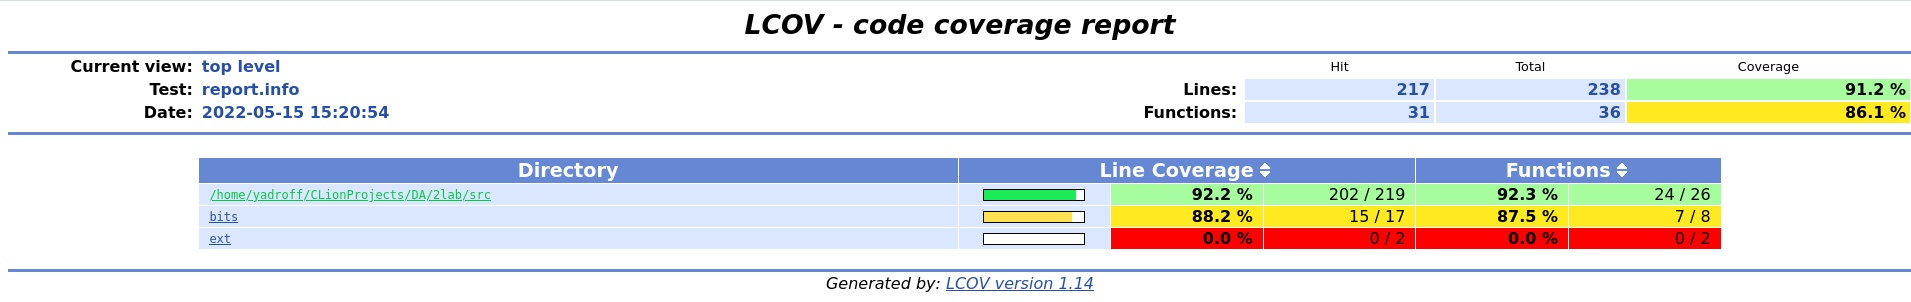
\includegraphics[width=\linewidth]{gcov1.jpg}
	\end{center}
	\begin{center}
		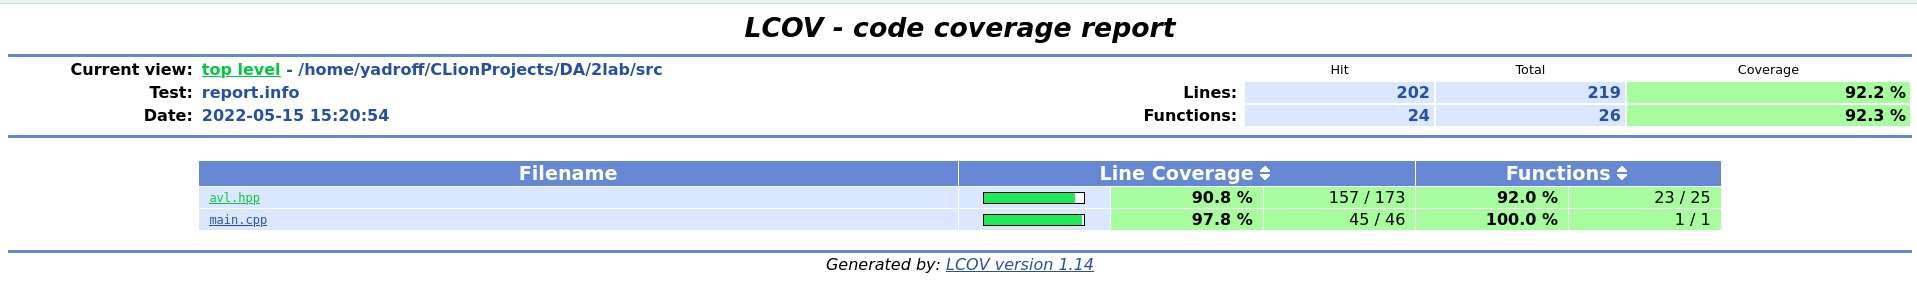
\includegraphics[width=\linewidth]{gcov2.jpg}
	\end{center}
	
	\begin{center}
		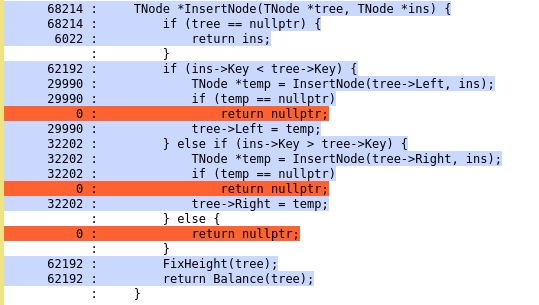
\includegraphics[width=\linewidth]{gcov3.jpg}
	\end{center}
	\begin{center}
		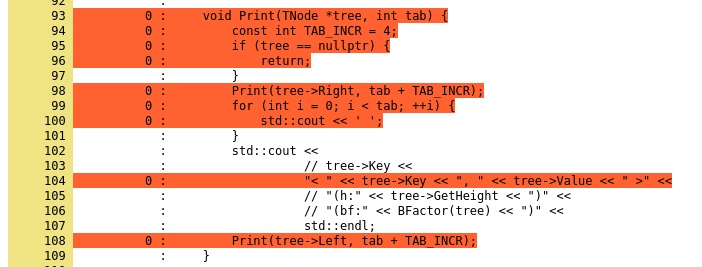
\includegraphics[width=\linewidth]{gcov4.jpg}
	\end{center}

	Как мы видим, в реализации avl-дерева покрыто $90.8\%$ кода, в то время как в main.cpp покрыто $97.8\%$ кода. Это объясняется тем, что в avl.hpp присутствует реализация печати дерева, а в main.cpp присутствует вызов этой печати. В тестах печать не использовалась, так как была заложена мной как служебная функция для проверки программы на правильность.
	
	 
	
	\subsection*{Выводы}
	
	Я познакомился с очень полезными инструментами:
	\begin{enumerate}
		\item Valgrind позволяет выявлять утечки памяти и профилировать код. Но для поиска утечек лучше использовать fsanitize, а для профилирования - утилиты ниже. Однако, инструмент довольно неплохо справляется со своей задачей.
		\item gprof позволяет оценить производительность программы, выявляя слабые места в плане производительности. Также есть функция постройки графа вызовов.
		\item gcov позволяет исследовать покрытие кода. Можно сгенерировать страницу формата html, в которой будет показано наше покрытие.
	\end{enumerate}
	Инструменты являются полезными. В дальнейшем будущем я буду стараться использовать их как можно чаще.
\end{document}
